\documentclass[11pt,letterpaper]{article}
\usepackage[margin=0.8in]{geometry}
\usepackage{graphicx,hyperref,float,caption,array}
\hypersetup{colorlinks=true,urlcolor=blue}
\setlength{\parindent}{0pt}
\setlength{\parskip}{0.5em}
\newcommand{\evidence}[2]{\begin{figure}[H]\centering\includegraphics[width=\linewidth,height=0.71\textheight,keepaspectratio]{#1}\caption{#2}\end{figure}}
\begin{document}
\begin{center}
{\Large\bfseries Machine Learning Operations}\\[0.3em]
{\large\bfseries FastAPI Lab: Wine Cultivar Prediction Service}
\end{center}
\textbf{Name:} Allen Febi Mariaantony Alphonsa\\
\textbf{Email:} \href{mailto:mariaantonyalphons.a@northeastern.edu}{mariaantonyalphons.a@northeastern.edu}\\
\textbf{Date:} October 27, 2026

\section*{Setup and Project Idea}
I adapted the model-serving workflow from Ramin Mohammadi's FastAPI lab into a wine cultivar prediction service. The original example uses a decision tree with the Iris dataset. My project uses chemical measurements to predict one of three wine cultivar classes, and adds batch processing, file uploads, saved history, background jobs, and monitoring.

I ran the application with Docker inside Ubuntu 22.04 in UTM. The container uses Python 3.12, FastAPI 0.115.12, Uvicorn 0.34.2, Pydantic 2.11.4, and scikit-learn 1.6.1. The complete dependency versions are saved in \path{requirements.lock.txt}. I opened Swagger UI in Zen through an SSH tunnel from Mac port 8005 to Ubuntu port 8004. These are local demonstration ports.

\section*{Training and Results}
I loaded scikit-learn's Wine recognition dataset: 178 samples, 13 numeric features, and three classes. I used a stratified split with 133 training records and 45 test records, using seed 42. A random forest with 200 trees was fitted only on the training data and saved with its feature order, class names, and evaluation metadata. I did not tune its settings on the test set.

\begin{center}
\begin{tabular}{lr}
\hline
\textbf{Held-out measurement} & \textbf{Result}\\\hline
Correct predictions & 45/45\\
Accuracy & 100\%\\
Macro F1 & 1.0000\\
Class 0 / 1 / 2 correct & 15 / 18 / 12\\\hline
\end{tabular}
\end{center}
I also sent all 45 held-out samples through the running Ubuntu API and obtained the same classifications. This is a small educational dataset and one fixed split; the result does not establish performance on new real-world wine samples. The labels are \texttt{class\_0}, \texttt{class\_1}, and \texttt{class\_2}, not wine quality scores or named grape varieties.

\section*{What I Added}
I extended the lab beyond a single prediction endpoint. The service has 12 API operations covering single, JSON-batch, and CSV predictions; history retrieval, filtering, pagination, annotation, and deletion; job creation and status; health; model metadata; and request counters. SQLite stores history in a Docker volume. FastAPI's lifespan loads the model once, \texttt{Depends} supplies it to handlers, and middleware adds request IDs and processing times.

\clearpage
\section*{Screenshot 1 -- Expanded Swagger Documentation}
I opened \url{http://localhost:8005/docs} in Zen. Swagger groups the routes by purpose and documents request and response schemas. GET retrieves data, POST creates predictions or jobs, PATCH changes a saved note, and DELETE removes a saved prediction.
\evidence{01-routes.png}{Swagger UI showing the prediction, history, background-job, health, model, and monitoring routes.}

\clearpage
\section*{Screenshot 2 -- Prediction and Response Headers}
I expanded \texttt{POST /predict}, clicked \textit{Try it out}, pasted the held-out sample from \path{evidence/sample.json}, and clicked \textit{Execute}. The endpoint returned HTTP 200, cultivar \texttt{class\_0}, and class probabilities 0.935, 0.040, and 0.025. The response also included a saved prediction ID.

The middleware added \texttt{X-Request-ID} and \texttt{X-Process-Time-Ms}. The screenshot shows 38.297 ms for that particular request. This is an individual observation, not a latency benchmark. The probabilities describe the fitted model's output and are not calibrated guarantees.
\evidence{02-prediction.png}{Successful live prediction, saved record ID, model version, processing time, and request ID in Zen.}

\clearpage
\section*{Screenshot 3 -- Validation and Error Handling}
I changed the sample's alcohol measurement to \texttt{-1} while leaving the other fields valid. Pydantic rejected it with HTTP 422 and identified the alcohol field. My exception handler returned a clear message and the request ID, which matched the response header. Invalid requests do not create prediction records.

All 13 feature fields are required and must contain finite positive numbers. Unexpected fields are rejected. Missing or wrongly typed values also return 422. These checks catch malformed input; they do not detect every unusual or out-of-distribution sample.
\evidence{03-validation.png}{HTTP 422 for a negative alcohol value, including the field-level explanation and matching request ID.}

\clearpage
\section*{Batch, CSV, History, and Background Work}
I tested the additional routes against the running service and saved their actual requests' status codes and response bodies in \path{evidence/live-api.json}.
\begin{center}
\begin{tabular}{p{0.63\linewidth}l}
\hline
\textbf{Action} & \textbf{Observed result}\\\hline
Submit two samples to \texttt{/predict/batch} & 200, two predictions\\
Upload a two-row CSV to \texttt{/predict/csv} & 200, two predictions\\
Filter history by class with limit and offset & 200, paged results\\
PATCH a saved record's note & 200, updated note\\
DELETE a saved record, then GET it & 204, then 404\\
Submit a background batch to \texttt{/jobs} & 202, job accepted\\
Poll its status URL & 200, completed\\\hline
\end{tabular}
\end{center}
JSON and CSV batches accept 1--100 samples; CSV files are limited to 1 MB and require the 13 exact feature headers. The entire input is validated before inference begins. BackgroundTasks returns an accepted response before running the job; its status and results are saved in SQLite.
\begin{figure}[H]\centering
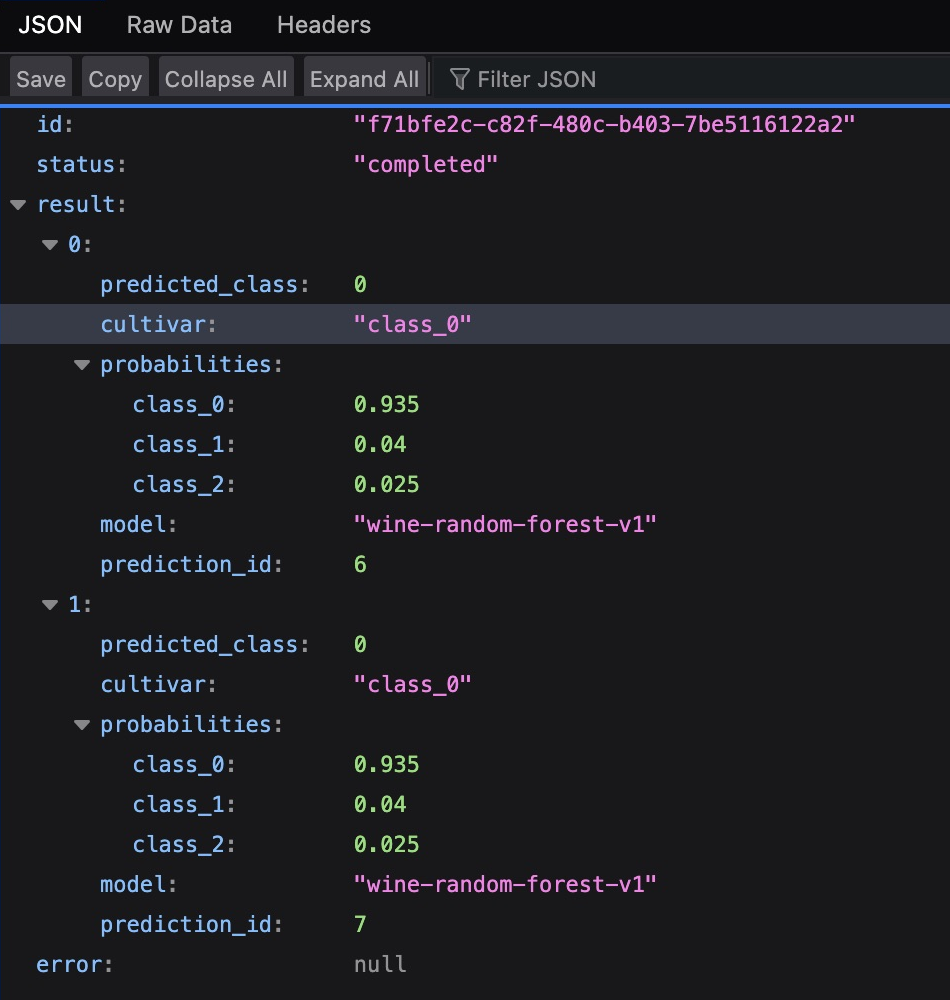
\includegraphics[width=0.62\linewidth,height=0.42\textheight,keepaspectratio]{05-job.png}
\caption{A completed background job in Zen with two prediction results and no error.}
\end{figure}
This is a single-worker learning service. BackgroundTasks is in-process, not a durable distributed queue. Restart recovery marks unfinished jobs as failed. A failure during inference can leave earlier results saved. Request counters reset when the process restarts; prediction history persists in the Docker volume. I verified history survived a container restart.

\clearpage
\section*{Screenshot 4 -- Ubuntu Verification}
All 22 tests passed inside the Ubuntu Docker container. They cover predictions, feature ordering, invalid inputs, batch limits, CSV upload and size limits, rejection before partial writes for invalid batches, history filtering and CRUD, background-job success and failure, restart recovery, persistence, headers, metrics, and OpenAPI docs. The dependency check found no broken requirements. Pytest reported one dependency deprecation warning from the Starlette test client.
\evidence{04-ubuntu.png}{Ubuntu terminal showing a healthy container, 22 passing tests, dependency verification, health response, and monitoring counters.}

\section*{How to Run}
From the repository folder:
\begin{verbatim}
docker compose up --build -d
docker compose exec -T api python -m pytest -q
python verify_live.py http://localhost:8004
\end{verbatim}
The last command needs the Python dependencies installed locally; alternatively run the requests in Swagger. On the same machine, open \url{http://localhost:8004/docs}. To run without Docker, create a Python 3.12 virtual environment, install \path{requirements.lock.txt}, run \texttt{python -m src.train}, then \texttt{uvicorn src.main:app --port 8004}. Use \texttt{docker compose stop} to stop the service while keeping its saved history.

\section*{Repository and References}
\textbf{Code, report, and verification evidence:}\\
\url{https://github.com/all3n2601/fastapi-wine-lab}

\textbf{Original lab:} \href{https://github.com/raminmohammadi/MLOps/tree/main/Labs/API_Labs/FastAPI_Labs}{Ramin Mohammadi's MLOps FastAPI Lab}. Its CC0 license is retained.\\
\textbf{Dataset:} \href{https://scikit-learn.org/stable/datasets/toy_dataset.html#wine-recognition-dataset}{scikit-learn Wine recognition dataset}.\\
\textbf{FastAPI docs:} \href{https://fastapi.tiangolo.com/tutorial/request-files/}{file uploads}, \href{https://fastapi.tiangolo.com/tutorial/dependencies/}{dependencies}, and \href{https://fastapi.tiangolo.com/tutorial/background-tasks/}{background tasks}.

\end{document}
